\begin{figure}[H]
    \centering
    \begin{subfigure}{0.1\textwidth} \raisebox{0.5\height}{\fbox{\includegraphics[width=\linewidth]{data/more_heat/0.png}}}  \caption{} \end{subfigure}
    
    \vspace{4mm}
    
    \begin{subfigure}{0.24\textwidth}
        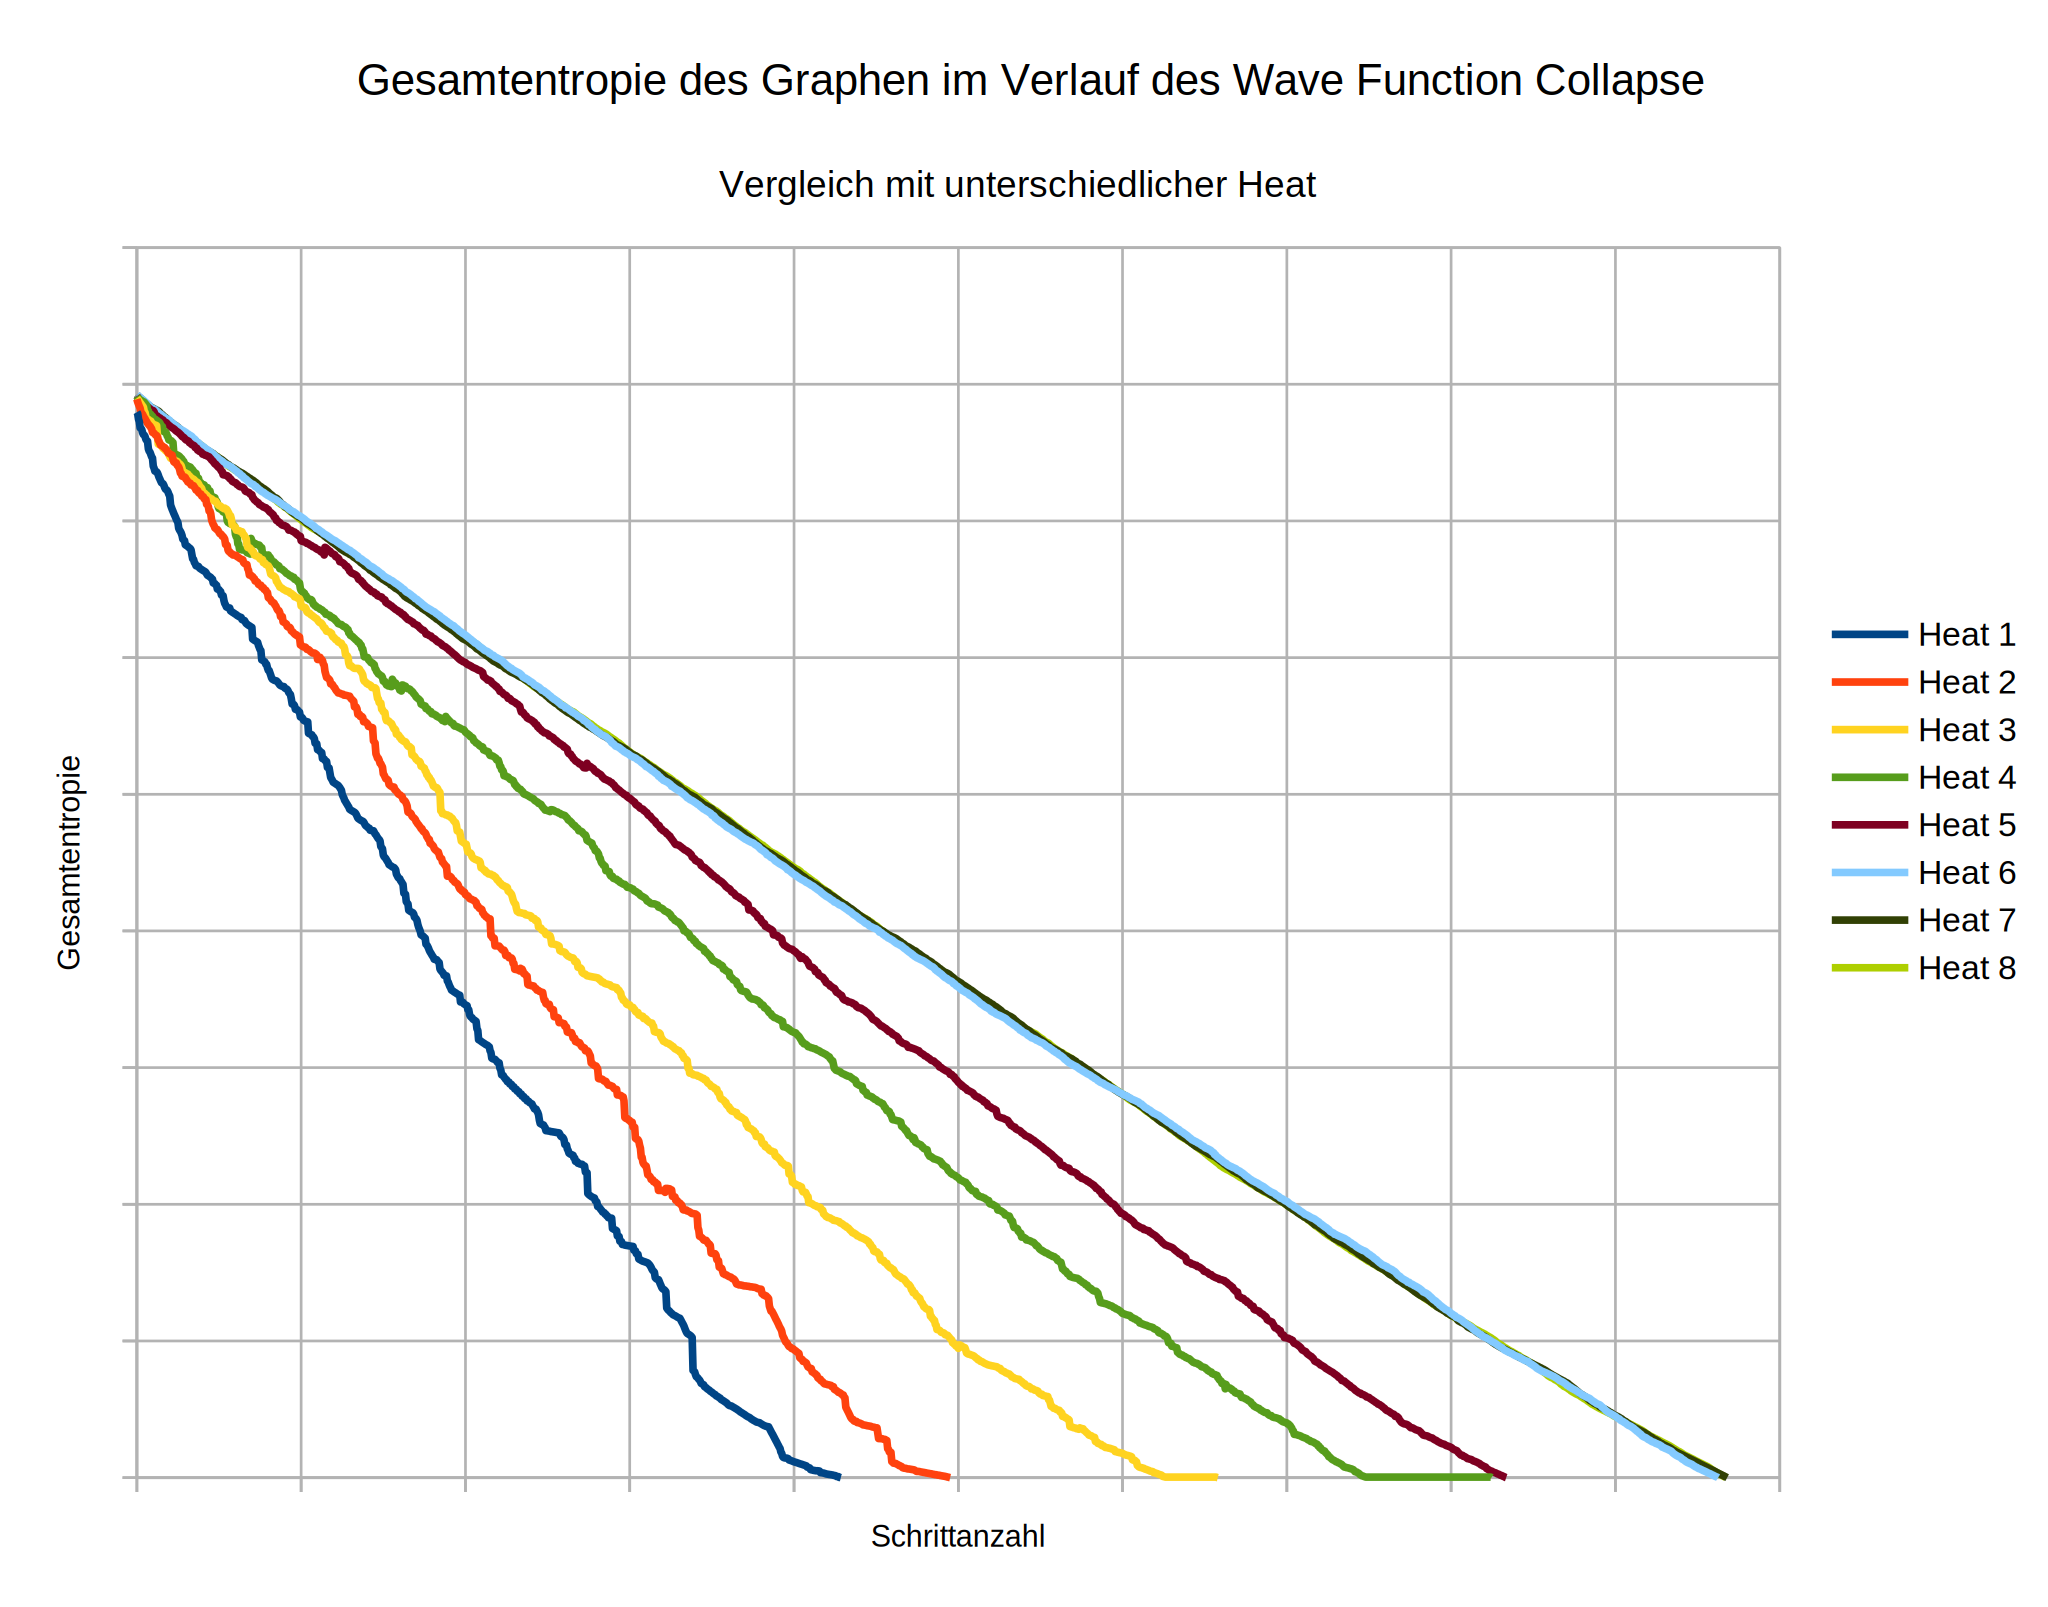
\includegraphics[width=\linewidth]{data/more_heat/1.png} \caption{Heat=1}
    \end{subfigure}
    \begin{subfigure}{0.24\textwidth}
        \includegraphics[width=\linewidth]{data/more_heat/2.png} \caption{Heat=2}
    \end{subfigure}
    \begin{subfigure}{0.24\textwidth}
        \includegraphics[width=\linewidth]{data/more_heat/3.png} \caption{Heat=3}
    \end{subfigure}
    \begin{subfigure}{0.24\textwidth}
        \includegraphics[width=\linewidth]{data/more_heat/4.png} \caption{Heat=4}
    \end{subfigure}
        
    \vspace{4mm}
    
    \begin{subfigure}{0.24\textwidth}
        \includegraphics[width=\linewidth]{data/more_heat/5.png} \caption{Heat=5}
    \end{subfigure}
    \begin{subfigure}{0.24\textwidth}
        \includegraphics[width=\linewidth]{data/more_heat/6.png} \caption{Heat=6}
    \end{subfigure}
    \begin{subfigure}{0.24\textwidth}
        \includegraphics[width=\linewidth]{data/more_heat/7.png} \caption{Heat=7}
    \end{subfigure}
    \begin{subfigure}{0.24\textwidth}
        \includegraphics[width=\linewidth]{data/more_heat/8.png} \caption{Heat=8}
    \end{subfigure}
    
    \caption{
        Beispiele der Generierung bei höherer Heat.
    }
    \label{fig:more_heat}
\end{figure}